\documentclass[a4paper]{article}
%\documentclass[8pt]{report}
%%%%%%%% CREATE DOCUMENT STRUCTURE %%%%%%%%
%% Language and font encodings
\usepackage[english]{babel}
\usepackage[utf8x]{inputenc}
\usepackage[T1]{fontenc}

%\usepackage{subfig}

%% Sets page size and margins
\usepackage[a4paper,top=3cm,bottom=2cm,left=2cm,right=2cm,marginparwidth=1.75cm]{geometry}

%% Useful packages
\usepackage{amsmath}
\usepackage{graphicx}
\usepackage[colorinlistoftodos]{todonotes}
\usepackage[colorlinks=true, allcolors=blue]{hyperref}
%\usepackage{caption}
\usepackage[justification=centering]{caption}
\usepackage{subcaption}
\usepackage{sectsty}
\usepackage{float}
\usepackage{titling} 
\usepackage{blindtext}
\usepackage[square,sort,comma,numbers]{natbib}
\usepackage[colorinlistoftodos]{todonotes}
\usepackage{xcolor}
\usepackage{fancyhdr}
\usepackage{lipsum}

%% definitions 
\definecolor{darkgreen}{rgb}{0.0, 0.4, 0.0}

%% Define your personal info here %%%%%%%%%%%%%%%%%%%%%%%
\newcommand\TPid{1}
\newcommand\TPname{Graphical rdfs - Marché de Carouge}
\newcommand\Firstname{Joao Filipe}
\newcommand\Familyname{Costa da Quinta}
\newcommand\Email{Joao.Costa@etu.unige.ch}
\newcommand\Firstnames{Léa}
\newcommand\Familynames{Heiniger}
\newcommand\Emails{Joao.Costa@etu.unige.ch}

%%%%%%%%%%%%%%%%%%%%%%%%%%%%%%%%%%%%%%%%%%%%%%%%%%%%%%%

%%%%%%% Page header %%%%%%
\pagestyle{fancy}
\fancyhf{}
\rhead{TP \TPid: \TPname}
\lhead{\Firstname \Familyname}
\rfoot{Page \thepage}


%%%%%%%% DOCUMENT %%%%%%%%
\begin{document}

%%%% Title Page
\begin{titlepage}

\newcommand{\HRule}{\rule{\linewidth}{0.5mm}} 							% horizontal line and its thickness

\center 
 
% University
\textsc{\LARGE Université de Genève}\\[1cm]

% Document info
\textsc{\Large Technologies du web sémantique}\\[0.2cm]									% Course Code
\HRule \\[0.8cm]
{ \huge \bfseries TP \TPid : \TPname}\\[0.7cm]								% Assignment
\HRule \\[2cm]
\large
\emph{Author:} \Firstnames \  \Familynames\\[0.5cm]		
\emph{E-mail:} {\color{blue}\Emails}\\[0.5cm]
\emph{Author:} \Firstname \  \Familyname\\[0.5cm]		
\emph{E-mail:} {\color{blue}\Email}\\[6cm]	

% Author info
% Author info
{\large \today}\\[2cm]

\includegraphics[width=0.4\textwidth]{images/unige_csd.png}\\[1cm] 	% University logo
\vfill 
\end{titlepage}


% ============================================
% ----------------------------------
\newpage
\section*{Introduction}
The goal of this project is to make a description of a tourist area using URI data. To do this we must integrate data from various sources, mainly Open Street Map and DBpedia.\\\\

\subsection*{Selected Area}
For this project we choose, Place du Marché Carouge. This a location that is full of life and incredible locations of leisure, there are very nice cafés, bars, restaurants and even a cinema. This locations is also very well located in the heart of the Commune de Carouge in Geneva, and it has near access to public transportation, so that anyone can access it easily. \\\\ For more detailed overview of the attractions of Place du Marché Carouge, one simply has to see the initial RDF schema in the next section !

\subsection*{Initial RDF schema}
\begin{figure}[H]
\center
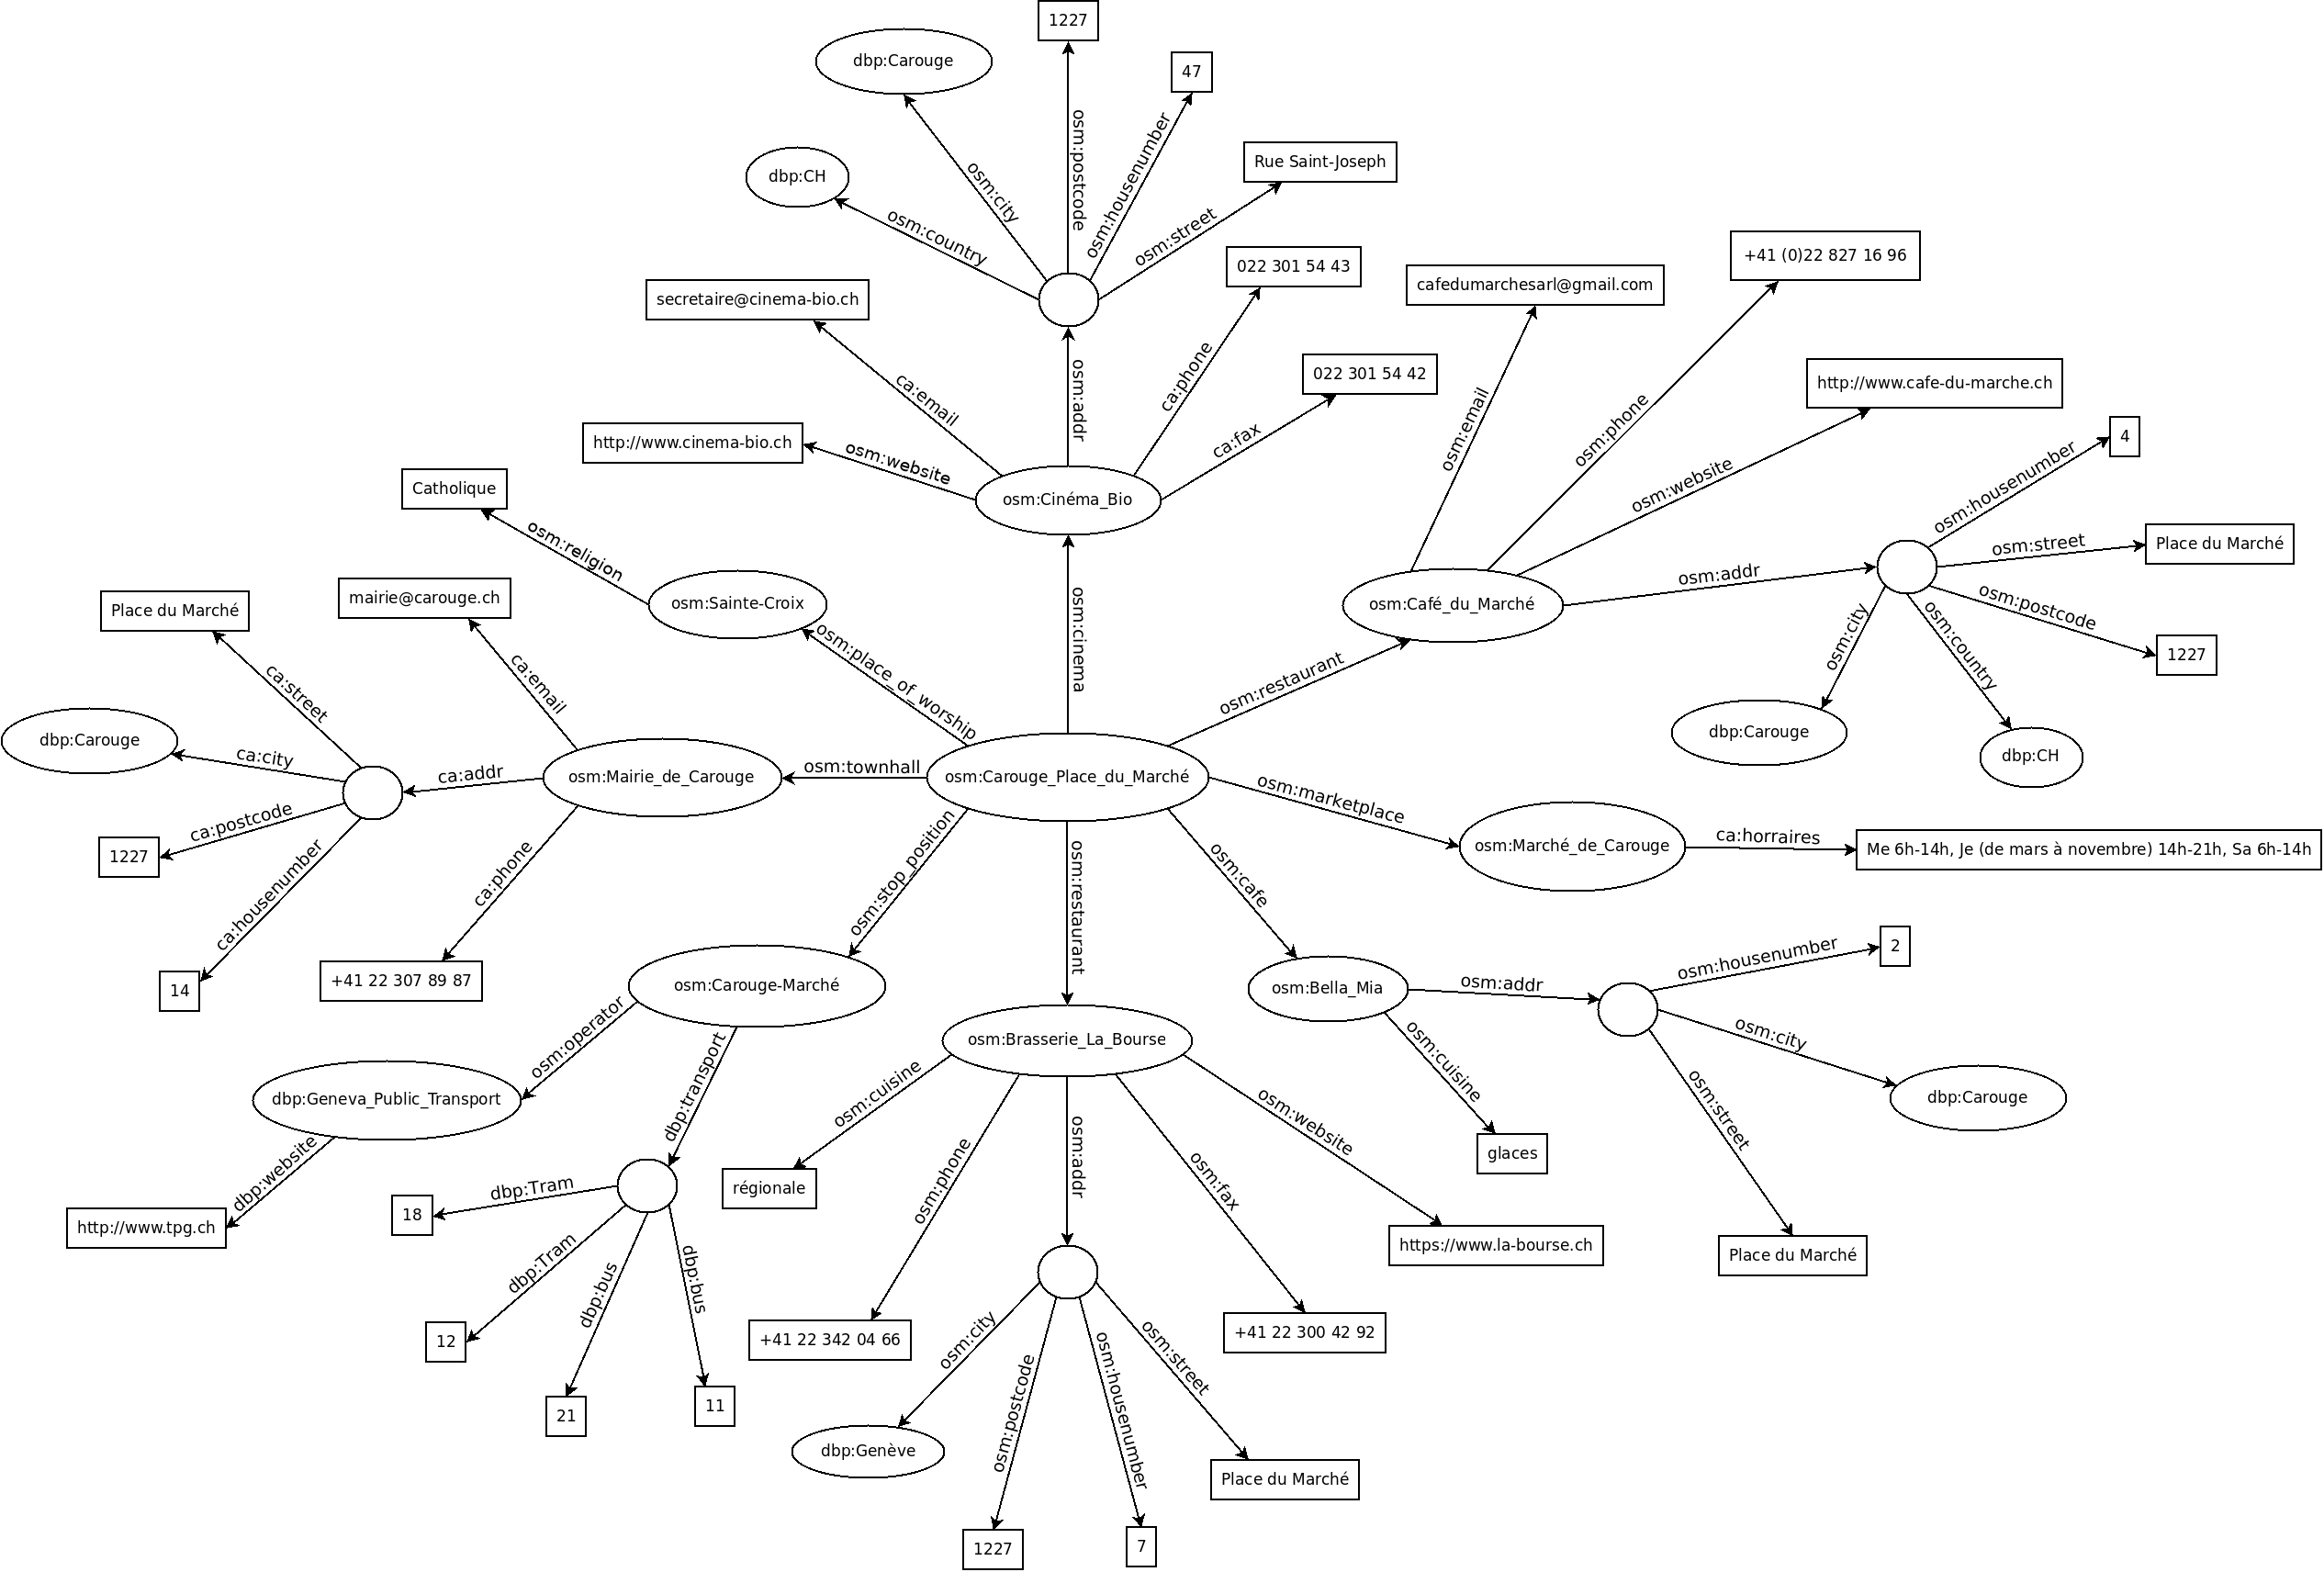
\includegraphics[width=1\textwidth]{images/Graph.PNG}
\caption{Initial RDF schema}
\end{figure}
\subsection*{Data sources}
To get all of the required information, we used OSM, which actually was full of information about the location we choose, this made our job easier, as we didn't have very large data to integrate from different sources. Any gaps that were left, were filled by using DBPedia, as well as the official web site of the Ville de Carouge.\\\\ With all three sources together we were able to fill our initial RDF schema with information.

\subsection*{GraphDB}

\end{document}
